\documentclass[8pt,a4paper,ngerman]{scrartcl}
\usepackage[utf8]{inputenc}
\usepackage{hyperref}
\usepackage{geometry}
\usepackage{graphicx}
\usepackage{pdfpages}
\geometry{a4paper, top=20mm, left=30mm, right=30mm, bottom=20mm, headsep=10mm, footskip=12mm}

\begin{document}
\thispagestyle{empty}
\begin{center}
    \LARGE{\textbf{Exposé zur Projekt- und Bachelorarbeit}}
\end{center}
\begin{center}
    \large{Christoph Piechula}
\end{center}
\begin{center}
    \small{\today}
\end{center}

\section{Motivation}
Für Film-Metadaten gibt es heutzutage verschiedene Online Quellen, welche sich
jedoch im Umfang, Qualität und Art der angebotenen Metadaten unterscheiden.
Die Motivation ist es eine modulare Open Source Library zu erstellen, die über
eine einheitliche Schnittstelle auf verschiedenen Metadatenanbieter (sog.
Provider) zugreifen kann und gleichzeitig leicht erweiterbar ist.  Desweiteren
soll auch das Zieldatenformat (\textit{json}, \textit{xml}) erweiterbar sein. 

Mit Hilfe der Library soll untersucht werden, wie gut sich Film-Metadaten
(insbesondere Filmbeschreibungen) extrahieren, analysieren und verarbeiten
lassen um dadurch z.B. Filme vergleichbar zu machen oder sogar Empfehlungen
aussprechen zu können. Zu den Zielgruppen gehören Media Center und Movie
Management/Tagging Tools Entwickler.

\section{Themenstellung}
Erstellung einer modularen Softwarebibliothek, welche verschiedene Arten von
Metadaten (Titel, Jahr, Handlung, Cover, Poster, etc.) über sog.  Provider von
verschiedenen Quellen holen kann. Mögliche Provider für Metadaten wären z.B.:
\begin{itemize}
    \item \url{www.tmdb.org} (allg. Metadaten, Filmbeschreibungen)
    \item \url{www.imdb.com} (allg. Metadaten, Filmbeschreibungen)
    \item \url{www.ofdb.de} (allg. Metadaten, Filmbeschreibungen, deutsche Sprache)
    \item \url{www.wikipedia.org} (Filmbeschreibungen, u.a.)
\end{itemize}
Die Bibliothek soll neben den Metadata Providern auch Output Converter für das
Ausgabeformat bieten. 
\\
Im zweiten Teil der Arbeit geht es darum, zu erforschen wie gut sich Film
Metadaten und Filmplot automatisiert verarbeiten lassen, um Informationen für z.B.
Empfehlungen ähnlicher Filme zu gewinnen. 

\subsection{Namensgebung:}
Die Library soll \emph{libhugin} heißen, wie Odin's Rabe \emph{Hugin}:
\begin{quote}
    \textit{Hugin gehört zum altnordischen Verb huga (denken), das hierzu zu
    stellende Substantiv hugi (Gedanke, Sinn) ist seinerseits die Grundlage für
    den Namen Hugin, der mit dem altnordischen Schlussartikel –in gebildet wurde.
    Hugin bedeutet folglich ,,der Gedanke''}
\end{quote}
Siehe auch: \url{http://de.wikipedia.org/wiki/Hugin\_und\_Munin}

\section{Geplantes Vorgehen}
Die Library soll in Python als Prototyp implementiert werden. Den Grundstein
bildet der \emph{libhugin-core} der Library, welcher für das Beschaffen der
Metadaten (Titel, Jahr, Genre, Filmbeschreibung) verschiedenen Quellen
zuständig sein soll.
\\
\\
Darauf aufbauend sollen die gesammelten Metadaten untersucht werden. Hierbei
soll die Library um \emph{libhugin-analyze} erweitert werden. Mögliche Ansätze und
Implementierungen hierbei:
\begin{itemize}
    \item Extraktion von Schlüsselwörtern (Analyse des Filmplots)
    \item Clustering von Filmen anhand Genre
    \item Clustering von Filmen anhand Schauspieler-Set
    \item Clustering von Filmen anhand extrahierten ,,Keywords''
\end{itemize}
Es soll ermittelt werden wie gut sich anhand der neu gewonnen
Informationen Filme vergleichen lassen und welche unterschiedlichen Kriterien
eine Rolle beim Vergleich von Filmen spielen. 
\\
\\
Anschließend sollen in der Bachelorarbeit die gewonnenen Erkenntnisse dargestellt
werden. 

\section{Aufteilung/Zeitplanung}
\paragraph{Projektarbeit:}
\begin{enumerate} 
    \item Implementierung von \emph{libhugin-core} (30\%)
    \item Implementierung von \emph{libhugin-analyze} (30\%)
    \item (Optional) Beispielanwendung oder Integration in ein
        bestehendes Projekt (10\%)
\end{enumerate}

\paragraph{Bachelorarbeit:}
\begin{enumerate} 
    \item Beschreibung der Theorie/Algorithmik mit Visualisierungen und
        Zusammenfassung der Forschungsergebnisse des Analyseparts der
        Library. (25\%)
    \item (Optional) Erweiterung der Beispielanwendung (5\%)
\end{enumerate}
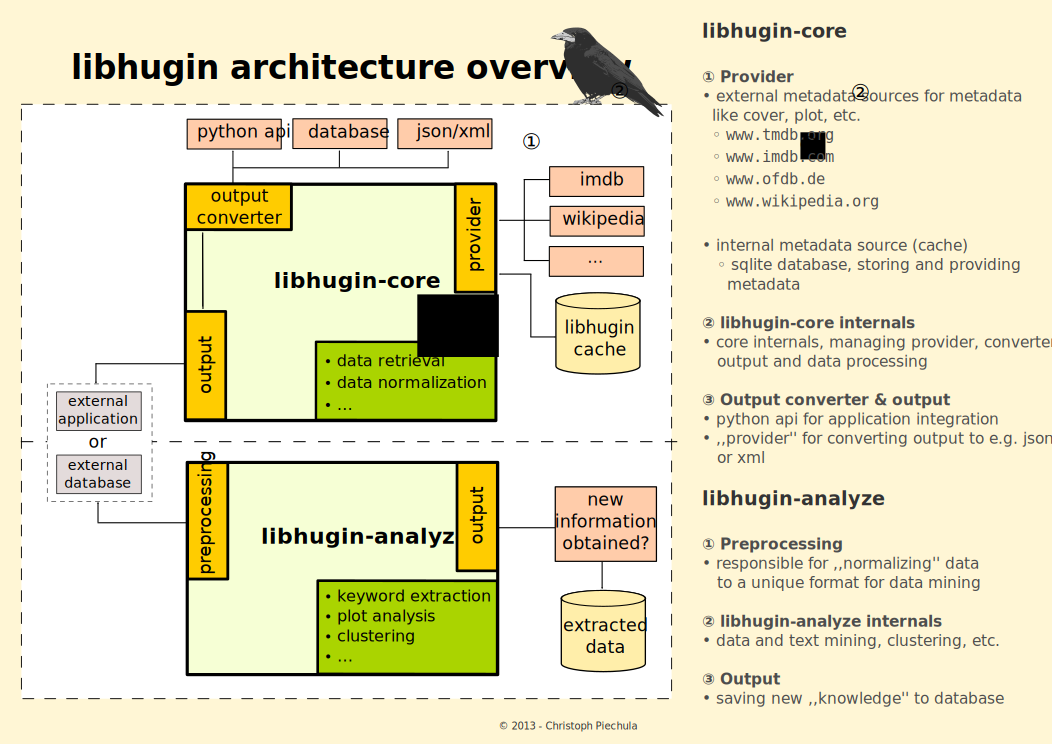
\includepdf{libhugin_arch.pdf}
\end{document}
